\documentclass[aspectratio=169]{beamer}
\mode<presentation>{
\usetheme{default}
}

\usepackage{graphicx} 
\usepackage{booktabs} 
\usepackage{graphicx,color}
\usepackage{minted} %extrai python com sitaxe destacada
\usepackage{pgfplots}
\usepackage{tikz}

\title[Short title]{Theano} 
\subtitle{Intel-Unesp/NCC - Machine Learning and High Performance Computing Team}
\subtitle{Hands-On}
\author{Machine Learning Team}

\begin{document}
\begin{frame}
\titlepage 
\end{frame}

%-S0
\begin{frame}
\frametitle{Test 01:Creating Variables }
Execute this code:
\\[0.5cm]
\inputminted{python}{./aux_files/th0.py}
\end{frame}
%-S0

%-S1
\begin{frame}
\frametitle{Test 02:Adding Matrices }
Evaluate the function : 
\\[0.5cm]
\inputminted{python}{./aux_files/th1.py}
\end{frame}
%-S1

%-S2
\begin{frame}
\frametitle{Test 03:Evaluating the Logistic Function }
Evaluate the function :
\\[0.5cm]
\inputminted{python}{./aux_files/th2.py}
\end{frame}
%-S2

%-S3
\begin{frame}
\frametitle{Test 04: Functions with Multiple Outputs }
Run this code and analyze its results :
\\[0.5cm]
\inputminted{python}{./aux_files/th3.py}
\end{frame}
%-S3

%-S4
\begin{frame}
\frametitle{Test 05:Computing the Gradient }
\inputminted{python}{./aux_files/th4.py}
\end{frame}
%-S4

%-S5
\begin{frame}
\frametitle{Theano: Math Challenge}
Let's compute the gradients of Logistic Curve
\\[0.1cm]
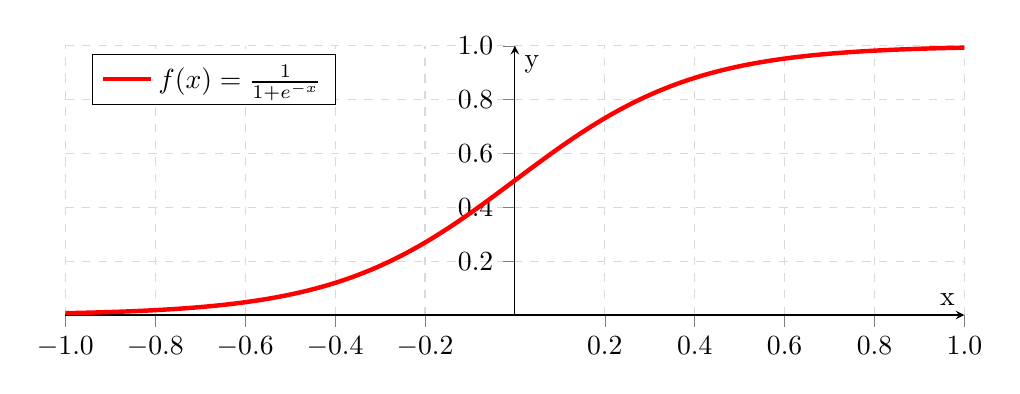
\begin{tikzpicture}
    \begin{axis}[
        legend pos=north west,
        axis x line=middle,
        axis y line=middle,
        x tick label style={/pgf/number format/fixed,
                            /pgf/number format/fixed zerofill,
                            /pgf/number format/precision=1},
        y tick label style={/pgf/number format/fixed,
                            /pgf/number format/fixed zerofill,
                            /pgf/number format/precision=1},
        grid = major,
        width=13cm,
        height=5cm,
        grid style={dashed, gray!30},
        xmin=-1,     % start the diagram at this x-coordinate
        xmax= 1,    % end   the diagram at this x-coordinate
        ymin= 0,     % start the diagram at this y-coordinate
        ymax= 1,   % end   the diagram at this y-coordinate
        %axis background/.style={fill=white},
        xlabel=x,
        ylabel=y,
        tick align=outside,
        enlargelimits=false]
        % plot the stirling-formulae
        \addplot[domain=-1:1, red, ultra thick,samples=500] {1/(1+exp(-5*x))};
        \addlegendentry{$f(x)=\frac{1}{1+e^{-x}}$}
    \end{axis}
\end{tikzpicture}
\\[0.3cm]
Hands On! - Write a code in Theano to find the Gradient of the Logistic and Hyperbolic Tangent Functions
- Plot the curves of both gradients and find out their outputs at x = -1.5, 0 and 1.5
\end{frame}
%-S5

\begin{frame}
\frametitle{References}
\footnotesize{
\begin{thebibliography}{99}
\bibitem[Theano - Online Theano Documentation]{p1} Theano  Documentation - http://deeplearning.net/software/theano/
\bibitem[Python Deep Learning]{p2} ZOCCA, V.; \textit{et.al.} Python Deep Learning. London:Packt Books, 2017


\end{thebibliography}
}
\end{frame}


\end{document}
